\documentclass[notheorems, hyperref={backref}]{beamer}

%% KEY LINES IN THIS TEX FILE %% (enter line number+gg to go)

%
% LOCAL FONT DEFINITIONS -- need to come first
%
%\usepackage{mathpazo}
\usepackage{libertine}
\usepackage[libertine]{newtxmath}
\usefonttheme[onlymath]{serif}
\usepackage{adjustbox}

%
% STANDARD PREAMBLE
%
%
% PACKAGES
%

\usepackage[T1]{fontenc}
% This uses 8-bit font encoding (with 256 glyphs) instead of the default 7-bit font encoding (with 128 glyphs). For example, with this option ö is a single glyph in the font, whereas on the 7-bit font encoding the font ö is made by adding an accent to the existing glyph o. A bad consequence of not using this package is that you cannot properly copy-paste such words form the output pdf file. Also, for some reason, funny stuff happens with |, < and > in text.

% Some people suggest to load fontenc before inputenc, most agree that it does not matter.

\usepackage[utf8]{inputenc}
% When you type ä in an editor set up for utf8, the machine stores the character number 228. When TeX reads the file it finds the character number 228 and the macros of inputenc transform this into \"a. Finally fontenc does its thing and transforms this into the command print character 228 (otherwise the two things would be printed separatedly as explained in fontenc).

\usepackage[UKenglish]{babel}
% To manage culturally determined typographical and similar rules, in this case for british english. Some people suggest to load babel after fontenc to avoid warnings, although most agree that it does not matter.

\usepackage{mathtools}
% Loads the amsmath package (\usepackage{amsmath}: miscellaneous improvements such as the commands \DeclareMathOperator and \text). It fixes some quirks it has and adds some useful settings, symbols and environments. It improves the aesthetics as well.

\usepackage{amssymb}
% Extended symbol collection, e.g. \Cap and \Cup. More importantly: the \mathbb command! It loads the amsfonts package (\usepackage{amsfonts}: fraktur letters, bold Greek letters...), so we do not need to include it in the preamble anymore.

\usepackage{mathrsfs}
% Font package (only supports upper case letters).

\usepackage{tikz}
\usetikzlibrary{shapes,arrows}

\usepackage{tikz-cd}
% To draw commutative diagrams.
\usetikzlibrary{decorations.markings}
% For open and closed immersions.
\usetikzlibrary{arrows,arrows.meta}
% To change the style of the arrows.
\tikzcdset{arrow style=tikz, diagrams={>=stealth}}

\usepackage{graphicx}
% An extension of the graphics package, with optional arguments for the \includegraphics command.

\usepackage{todonotes}
% To write to do notes use the command \todo.

% \usepackage{xcolor}
% To write in colors.
% Already loaded by beamer class.

\usepackage{mathdots}
% To draw diagonal dots.

\usepackage{marginnote}
% To write on margins.

\usepackage{tcolorbox}
% Color boxes.

\usepackage{manfnt}
% To draw dangerous bent symbol.

\usepackage{float}
% Improved interface for floating objects such as figures and tables, introducing for example the H modifier to force the position of a float in the page or the boxed float. Should be loaded before hyperref.

% \usepackage[backref]{hyperref}
% To handle cross-referencing and produce hypertext links in the document. It should be loaded last (with few exceptions), because it redefines many LaTeX commands.
% The backref option inserts links on each bibliography entry to the pages in which the citation was used.
%% The hidelinks option removes colors and boxes around links, but the links remain clickable. On firefox the links are even highlighted when the mouse pointer passes over them.
% \renewcommand{\backref}[1]{$\uparrow$~#1}
% Adds an upwards arrow before referencing to the pages in which the citations appear.
% Already loaded by beamer class.

\usepackage[noabbrev]{cleveref}
% Enhances cross-referencing features, e.g. to reference to a theorem and automatically include the word theorem.
% No abbreviature option to write figure instead of fig. etc.

% Open and closed immersion arrows.
\makeatletter
\tikzcdset{
open/.code={\tikzcdset{hook, circled};},
closed/.code={\tikzcdset{hook, slashed};},
circled/.code={\tikzcdset{markwith={\draw (0,0) circle (.375ex);}};},
slashed/.code={\tikzcdset{markwith={\draw[-] (-.4ex,-.4ex) -- (.4ex,.4ex);}};},
markwith/.code={
\pgfutil@ifundefined{tikz@library@decorations.markings@loaded}%
{\pgfutil@packageerror{tikz-cd}{You need to say %
\string\usetikzlibrary{decorations.markings} to use arrow with markings}{}}{}%
\pgfkeysalso{/tikz/postaction={/tikz/decorate,
/tikz/decoration={
markings,
mark = at position 0.5 with
{#1}}}}},
}
\makeatother

% Custom colors
\definecolor{darkgreen}{RGB}{0,75,0}
\definecolor{darkblue}{RGB}{0,0,75}
\definecolor{darkred}{RGB}{75,0,0}
\definecolor{linkred}{rgb}{0.6,0.2,0.2}
\definecolor{linkblue}{rgb}{0,0.2,0.6}
\definecolor{linkgreen}{rgb}{0.2,0.6,0.2}

% Limit table of contents to section titles
\setcounter{tocdepth}{1}

% Sloppy formatting -- often looks better
\sloppy

%
% FONT DEFINTIONS
%

% Script Font used for sheaves
\DeclareFontFamily{OMS}{rsfs}{\skewchar\font'60}
\DeclareFontShape{OMS}{rsfs}{m}{n}{<-5>rsfs5 <5-7>rsfs7 <7->rsfs10 }{}
\DeclareSymbolFont{rsfs}{OMS}{rsfs}{m}{n}
\DeclareSymbolFontAlphabet{\scr}{rsfs}
\DeclareSymbolFontAlphabet{\scr}{rsfs}

% Sheaves
\newcommand{\sA}{\scr{A}}
\newcommand{\sB}{\scr{B}}
\newcommand{\sC}{\scr{C}}
\newcommand{\sD}{\scr{D}}
\newcommand{\E}{\scr{E}} % Exception (Vector bundles)
\newcommand{\F}{\scr{F}} % Exception (Coherent sheaves)
\newcommand{\G}{\scr{G}} % Exception (Coherent sheaves)
\newcommand{\sH}{\scr{H}}
\renewcommand{\hom}{\scr{H}\negthinspace om} % Exception (Hom-sheaf)
\newcommand{\I}{\scr{I}} % Exception (Ideal sheaves)
\newcommand{\sJ}{\scr{J}}
\newcommand{\sK}{\scr{K}}
\renewcommand{\L}{\scr{L}} % Exception (Line bundles)
\newcommand{\M}{\scr{M}} % Exception (Line bundles)
\newcommand{\sN}{\scr{N}}
\renewcommand{\O}{\scr{O}} % Exception (Structure sheaf)
\newcommand{\sP}{\scr{P}}
\newcommand{\sQ}{\scr{Q}}
\newcommand{\sR}{\scr{R}}
\newcommand{\sS}{\scr{S}}
\newcommand{\sT}{\scr{T}}
\newcommand{\sU}{\scr{U}}
\newcommand{\sV}{\scr{V}}
\newcommand{\sW}{\scr{W}}
\newcommand{\w}{\omega} % Addition (Canonical sheaf)
\newcommand{\sX}{\scr{X}}
\newcommand{\sY}{\scr{Y}}
\newcommand{\sZ}{\scr{Z}}

% Mathcal fonts
\newcommand{\calA}{\mathcal{A}}
\newcommand{\calB}{\mathcal{B}}
\newcommand{\calC}{\mathcal{C}}
\newcommand{\calD}{\mathcal{D}}
\newcommand{\calE}{\mathcal{E}}
\newcommand{\calF}{\mathcal{F}}
\newcommand{\calG}{\mathcal{G}}
\newcommand{\calH}{\mathcal{H}}
\newcommand{\calI}{\mathcal{I}}
\newcommand{\calJ}{\mathcal{J}}
\newcommand{\calK}{\mathcal{K}}
\newcommand{\calL}{\mathcal{L}}
\newcommand{\calM}{\mathcal{M}}
\newcommand{\calN}{\mathcal{N}}
\newcommand{\calO}{\mathcal{O}}
\newcommand{\calP}{\mathcal{P}}
\newcommand{\calQ}{\mathcal{Q}}
\newcommand{\calR}{\mathcal{R}}
\newcommand{\calS}{\mathcal{S}}
\newcommand{\calT}{\mathcal{T}}
\newcommand{\U}{\mathcal{U}} % Exception (Open covers)
\newcommand{\calV}{\mathcal{V}}
\newcommand{\calW}{\mathcal{W}}
\newcommand{\X}{\mathcal{X}} % Exception (Families of varieties)
\newcommand{\Y}{\mathcal{Y}} % Exception (Families of varieties)
\newcommand{\calZ}{\mathcal{Z}}

% Blackboard Bold Symbols
\newcommand{\A}{\mathbb{A}} % Exception (Affine space)
\newcommand{\bbB}{\mathbb{B}}
\newcommand{\C}{\mathbb{C}} % Exception (Complex numbers)
\newcommand{\bbD}{\mathbb{D}}
\newcommand{\bbE}{\mathbb{E}}
\newcommand{\bbF}{\mathbb{F}}
\newcommand{\bbG}{\mathbb{G}}
\newcommand{\Gm}{\mathbb{G}_{\mathrm{m}}} % Addition (Punctured affine line)
\newcommand{\bbH}{\mathbb{H}}
\newcommand{\bbI}{\mathbb{I}}
\newcommand{\bbJ}{\mathbb{J}}
\newcommand{\bbK}{\mathbb{K}}
\renewcommand{\k}{\Bbbk} % Addition (Field)
\newcommand{\bbL}{\mathbb{L}}
\newcommand{\bbM}{\mathbb{M}}
\newcommand{\N}{\mathbb{N}} % Exception (Natural numbers)
\newcommand{\bbO}{\mathbb{O}}
\renewcommand{\P}{\mathbb{P}} % Exception (Projective space)
\newcommand{\Q}{\mathbb{Q}} % Exception (Rational numbers)
\newcommand{\R}{\mathbb{R}} % Exception (Real numbers)
\newcommand{\bbS}{\mathbb{S}}
\newcommand{\bbT}{\mathbb{T}}
\newcommand{\bbU}{\mathbb{U}}
\newcommand{\V}{\mathbb{V}} % Exception (Geometric vector bundle)
\newcommand{\bbW}{\mathbb{W}}
\newcommand{\bbX}{\mathbb{X}}
\newcommand{\bbY}{\mathbb{Y}}
\newcommand{\Z}{\mathbb{Z}} % Exception (Integers)

% Boldfont (categories)
\newcommand{\bfA}{\mathbf{A}}
\newcommand{\Ab}{\mathbf{Ab}}
\newcommand{\bfB}{\mathbf{B}}
\newcommand{\bfC}{\mathbf{C}}
\newcommand{\Cat}{\mathbf{Cat}} % Addition (Categories)
\newcommand{\Coh}{\mathbf{Coh}} % Addition (Coherent sheaves)
\newcommand{\D}{\mathbf{D}} % Exception (Derived category)
\newcommand{\Db}{\mathbf{D}^{\mathrm{b}}} % Addition (Bounded derived category)
\newcommand{\bfE}{\mathbf{E}}
\newcommand{\bfF}{\mathbf{F}}
\newcommand{\bfG}{\mathbf{G}}
\newcommand{\bfH}{\mathbf{H}}
\newcommand{\bfI}{\mathbf{I}}
\newcommand{\bfJ}{\mathbf{J}}
\newcommand{\K}{\mathbf{K}} % Exception (Homotopy category)
\newcommand{\bfL}{\mathbf{L}}
\newcommand{\bfM}{\mathbf{M}}
\newcommand{\Mod}{\mathbf{Mod}} % Addition (Modules)
\newcommand{\bfN}{\mathbf{N}}
\newcommand{\bfO}{\mathbf{O}}
\newcommand{\bfP}{\mathbf{P}}
\newcommand{\PSh}{\mathbf{PSh}} % Addition (Presheaves)
\newcommand{\bfQ}{\mathbf{Q}}
\newcommand{\QCoh}{\mathbf{QCoh}} % Addition (Quasi-coherent sheaves)
\newcommand{\bfR}{\mathbf{R}}
\newcommand{\bfS}{\mathbf{S}}
\newcommand{\Set}{\mathbf{Set}} % Addition (Sets)
\newcommand{\Sh}{\mathbf{Sh}} % Addition (Sheaves)
\newcommand{\bfT}{\mathbf{T}}
\renewcommand{\Top}{\mathbf{Top}} % Addition (Topological spaces)
\newcommand{\bfU}{\mathbf{U}}
\newcommand{\bfV}{\mathbf{V}}
\renewcommand{\Vec}{\mathbf{Vec}} % Addition (Vector bundles)
\newcommand{\bfW}{\mathbf{W}}
\newcommand{\bfX}{\mathbf{X}}
\newcommand{\bfY}{\mathbf{Y}}
\newcommand{\bfZ}{\mathbf{Z}}

% Mathfrak for ideals
\renewcommand{\a}{\mathfrak{a}}
\renewcommand{\b}{\mathfrak{b}}
\renewcommand{\c}{\mathfrak{c}}
\renewcommand{\d}{\mathfrak{d}}
\newcommand{\e}{\mathfrak{e}}
\newcommand{\m}{\mathfrak{m}}
\newcommand{\n}{\mathfrak{n}}

% Custom theorem styles (empty fields take default values)
\newtheoremstyle{darkgreentheorem}% name of the style
{}% measure of space to leave above the theorem. E.g.: 3pt
{}% measure of space to leave below the theorem. E.g.: 3pt
{\itshape}% name of font to use in the body of the theorem
{}% measure of space to indent
{\color{darkgreen}\bfseries}% name of head font
{}% punctuation between head and body
{ }% space after theorem head; " " = normal interword space
{}% Manually specify head
\newtheoremstyle{darkbluedefinition}
{}{}{}{}{\color{darkblue}\bfseries}{}{ }{}
\newtheoremstyle{darkredexample}
{}{}{}{}{\color{darkred}\bfseries}{}{ }{}



\allowdisplaybreaks

%
% ABOUT FONT DEFINTIONS IN THE PREAMBLE
%
% Mathscr for sheaves use \sA, where A can be any letter. Exceptions and additions:
% % \E (vector bundles)
% % \F (coherent sheaves)
% % \G (coherent sheaves)
% % \hom (sheaf hom)
% % \I (ideal sheaves)
% % \L (line bundles)
% % \M (line bundles)
% % \O (structure sheaf)
% % \w (canonical sheaf)
%
% Mathcal use \calA. Exceptions and additions:
% % \U (open cover)
% % \X (families of varieties)
% % \Y (families of varieties)
%
% Mathbb use \bbA. Exceptions and additions:
% % \A (affine space)
% % \C (complex numbers)
% % \Gm (puctured affine line)
% % \k (field)
% % \N (natural numbers)
% % \P (projective space)
% % \Q (rational numbers)
% % \R (real numbers)
% % \V (geometric vector bundle)
% % \Z (integers)
%
% Boldfont for categories use \bfA. Additions:
% % \Cat (categories)
% % \Coh (coherent sheaves)
% % \D (derived category)
% % \Db (bounded derived category)
% % \K (homotopy category)
% % \Mod (modules)
% % \PSh (presheaves)
% % \QCoh (quasi-coherent sheaves)
% % \Set (sets)
% % \Sh (sheaves)
% % \Top (topological spaces)
% % \Vec (vector bundles)
%
% Mathfrak for ideals
% % From \a to \e
% % \m and \n for maximal ideals

%
% THEOREM ENVIRONMENTS
%
% Theorems, propositions, etc (dark green)
\theoremstyle{darkgreentheorem}
\newtheorem{thm}{Theorem}
\newtheorem{lm}[thm]{Lemma}
\newtheorem{prop}[thm]{Proposition}
\newtheorem{cor}[thm]{Corollary}
\newtheorem{conj}[thm]{Conjecture}
% Definitions (dark blue)
\theoremstyle{darkbluedefinition}
\newtheorem{defn}[thm]{Definition}
% Examples (dark red)
\theoremstyle{darkredexample}
\newtheorem{exa}[thm]{Example}
% Remarks (black)
\theoremstyle{remark}
\newtheorem{rem}[thm]{Remark}
\newtheorem{nota}[thm]{Notation}
\newtheorem{fact}[thm]{Fact}
\newtheorem{q}[thm]{Question}
\newtheorem{pbl}[thm]{Problem}

%
% THEOREM CROSS-REFERENCING
%
\crefname{thm}{theorem}{theorems}
\Crefname{thm}{Theorem}{Theorems}
\crefname{lm}{lemma}{lemmas}
\Crefname{lm}{Lemma}{Lemmas}
\crefname{prop}{proposition}{propositions}
\Crefname{prop}{Proposition}{Propositions}
\crefname{cor}{corollary}{corollaries}
\Crefname{cor}{Corollary}{Corollaries}
\crefname{conj}{conjecture}{conjectures}
\Crefname{conj}{Conjecture}{Conjectures}
\crefname{defn}{definition}{definitions}
\Crefname{defn}{Definition}{Definitions}
\crefname{exa}{example}{examples}
\Crefname{exa}{Example}{Examples}
\crefname{rem}{remark}{remarks}
\Crefname{rem}{Remark}{Remarks}
\crefname{nota}{notation}{notations}
\Crefname{nota}{Notation}{Notations}
\crefname{fact}{fact}{facts}
\Crefname{fact}{Fact}{Facts}
\crefname{q}{question}{questions}
\Crefname{q}{Question}{Questions}
\crefname{pbl}{problem}{problems}
\Crefname{pbl}{Problem}{Problems}

%
% MATH OPERATORS
%
\DeclareMathOperator{\Hom}{Hom}
\DeclareMathOperator{\gr}{gr}
\DeclareMathOperator{\im}{im}

%
% OTHER COMMANDS
%
\newcommand{\ot}{\otimes}
\newcommand{\op}{\oplus}
\newcommand{\filt}{F^{\bullet}}

%
% TITLE PAGE INFORMATION
%
\title[Basic Notions --- Spectral Sequences]{Basic Notions --- Spectral Sequences}
\author{Pedro Núñez}
\institute{University of Freiburg}
\date{10th December 2020}
 
%
% LINKS AND PDF OPTIONS
%
\makeatletter
\hypersetup{
  %pdfauthor={\authors},
  pdftitle={\@title},
  %pdfsubject={\@subjclass},
  %pdfkeywords={\@keywords},
  %pdfstartview={Fit},
  %pdfpagelayout={TwoColumnRight},
  %pdfpagemode={UseOutlines},
  bookmarks,
  colorlinks,
  linkcolor=linkblue,
  citecolor=linkblue,
  urlcolor=linkblue}
\makeatother
\usecolortheme{orchid}
 
\begin{document}
 
\frame{\titlepage}

\begin{frame}
    \frametitle{\centerline{``You could have invented spectral sequences''\footnote{Title of the expository article \cite{cho06}}}}
    \begin{figure}
	\centering
	
\includegraphics[scale=.6]{pictures/good}
    \end{figure}
\end{frame}

\begin{frame}
    \frametitle{\centerline{Notation gets ugly very soon}}
    \begin{figure}
	\centering
	
\includegraphics[scale=.307]{pictures/bad}
    \end{figure}
\end{frame}

\begin{frame}
    \frametitle{Notation and conventions \cite{stacks}}
	\begin{itemize}
	    \item Only finite dimensional vector spaces over $\Q$ for simplicity.
		\pause
	    \item (Cochain) complexes denoted with capital letters $C$ and not $C^{\bullet}$.
		\pause
	    \item Cohomology again denoted just $H(C)$ and not $H^{\bullet}(C)$.
		\pause
	    \item Cohomology is regarded as a copmlex with $0$ differentials
		\[ H(C)=\bigoplus_{i\in \Z}H^{i}(C)[-i]:=\left(\cdots H^{-1}(C)\xrightarrow{0} H^{0}(C)\xrightarrow{0}H^{1}(C) \cdots \right). \]
		\pause
	    \item If it is clear to which $C$ we refer, denote $H(C)$ simply by $H$.
		\pause
	    \item (Decreasing) filtrations are always finite for simplicity:
		\[ F^{\bullet}A \colon \quad 0=F^{n}A\subseteq \ldots \subseteq F^{0}A=A. \]
		\pause
	    \item The graded object associated to a filtration $F^{\bullet}A$ is denoted
		\[ \gr{A}=\bigoplus_{p\in \N} \gr^{p}A:=\bigoplus_{p\in \N}\left( F^{p}A/F^{p+1}A \right). \]
	\end{itemize}
\end{frame}

\begin{frame}
    \frametitle{\textsc{Goal}: compute cohomology with the help of a filtration}
    % Define block styles
\tikzstyle{decision} = [diamond, draw, fill=red!20, 
    text width=2.5em, text badly centered, node distance=3cm, inner sep=0pt]
\tikzstyle{start} = [draw, rectangle, fill=blue!20, 
    text width=3em, text centered, rounded corners=3mm, minimum height=2em]
\tikzstyle{tbc} = [draw, ellipse, fill=blue!20, 
    text width=3em, text centered, minimum height=2em]
\tikzstyle{block} = [rectangle, draw, fill=yellow!20, 
    text width=4em, text centered, minimum height=2em]
\tikzstyle{result} = [draw, rectangle, fill=green!20, 
    text width=11em, text centered, rounded corners=3mm, minimum height=3em]
\tikzstyle{line} = [draw, -latex']
\tikzstyle{cloud} = [draw, trapezium, trapezium left angle=75, trapezium right angle=105, fill=red!20, node distance=3cm,
    minimum height=2em]
\begin{center}
\begin{tikzpicture}[node distance = 2cm, auto]
    % Place nodes
    \node [start] (complex) {$C$};
    \node [cloud, below of=complex, node distance=15mm] (filtration) {$F^{\bullet}C$};
    \node [block, left of=filtration, node distance=3cm] (gradedC) {$\gr^{p}C$};
    \node [block, right of=filtration, node distance=3cm] (induced) {$F^{\bullet}H$};
    \node [block, below of=gradedC, node distance=20mm] (cohomGradedC) {$H(\gr^{p}C)$};
    \node [block, below of=induced, node distance=20mm] (gradedH) {$\gr^{p}H$};
    \node [decision, below of=filtration, node distance=30mm] (compare) {$\cong $?};
    \node [start, below of=cohomGradedC, node distance=18mm] (whatNow) {TBC};
    \node [result, below of=compare, node distance=20mm] (cohom) {$H\cong \gr H \cong \bigoplus H(\gr^{p}C)$};
    % Draw edges
    \path [line] (complex) -- (filtration);
    \path [line] (filtration) -- (gradedC);
    \path [line] (filtration) -- (induced);
    \path [line] (gradedC) -- (cohomGradedC);
    \path [line] (induced) -- (gradedH);
    \path [line] (cohomGradedC) -| (compare);
    \path [line] (gradedH) |- (compare);
    \path [line] (compare) -- node {yes}(cohom);
    \path [line, dashed] (compare) -| node [near start] {no}(whatNow);
\end{tikzpicture}
\end{center}
\end{frame}

\begin{frame}
    \frametitle{Filtration induced in cohomology}
    A filtration on the complx $F^{\bullet}C$ induces a filtration in cohomology
    \[ F^{p}H:=\im(H(F^{p}C)\to H(C))\subseteq H(C)=H, \]
    where $H(F^{p}C)\to H(C)$ is induced by the inclusion map $F^{p}C\hookrightarrow C$.
\end{frame}

\begin{frame}
    \frametitle{\textsc{Baby Example}: 2 step filtration on a length 1 complex}
    \adjustbox{scale=1.2,center}{%
	\begin{tikzcd}[ampersand replacement=\&]
	    C \&[-20pt] \&[-15pt] \&[-15pt] \&[10pt] \&[-15pt] \&[-15pt] \\[-15pt]
	    F^{0}C\arrow[draw=none]{u}[sloped,auto=false]{=} \& \cdots\arrow{r} \& 0\arrow{r} \& C^{0}\arrow{r}{d^{0}} \arrow{r} \& C^{1}\arrow{r} \& 0\arrow{r} \& \cdots \\
	    F^{1}C\arrow[draw=none]{u}[sloped,auto=false]{\subseteq} \& \cdots\arrow{r} \& 0\arrow{r} \& F^{1}C^{0}\arrow[draw=none]{u}[sloped,auto=false]{\subseteq}\arrow{r}{d^{0}|_{F^{1}C^{0}}} \& F^{1}C^{1}\arrow[draw=none]{u}[sloped,auto=false]{\subseteq}\arrow{r} \& 0 \arrow{r} \&[-15pt]\cdots \\
	    F^{2}C\arrow[draw=none]{u}[sloped,auto=false]{\subseteq} \& \cdots\arrow{r} \& 0 \arrow{r} \& 0\arrow[draw=none]{u}[sloped,auto=false]{\subseteq}\arrow{r} \& 0\arrow[draw=none]{u}[sloped,auto=false]{\subseteq}\arrow{r}\& 0 \arrow{r} \&[-15pt]\cdots \\[-15pt]
	    0\arrow[draw=none]{u}[sloped,auto=false]{=} \& \& \& \& \& \&
	\end{tikzcd}
    }
\end{frame}

\begin{frame}
    \frametitle{\textsc{Baby Example}: filtration induced in cohomology}
    \vspace{-3mm}
    We first look at the map induced by $F^{1}C\hookrightarrow C$ in cohomology:

    \vspace{2mm}
    \adjustbox{scale=1.1,center}{%
	\begin{tikzcd}[ampersand replacement=\&]
	    \hspace{5mm}H(F^{1}C)\mbox{ }\mbox{ }\mbox{ }=\arrow{d} \&[-20pt] \hspace{2mm}\ker\left(d^{0}|_{F^{1}C}\right)[0]\op \left(\frac{F^{1}C^{1}}{\im\left(d^{0}|_{F^{1}C}\right)}\right)[-1]\arrow{d} \\
	    \hspace{7mm}H(C)\quad = \& \hspace{3.5mm}\ker(d^{0})[0]\op \left(\frac{C^{1}}{\im(d^{0})}\right)[-1]
	\end{tikzcd}
    }
    \pause
    
    \vspace{1cm}
    The filtration on cohomology was given by its image, hence
    \vspace{3mm}

    \adjustbox{scale=1.2,center}{%
    \begin{tcolorbox}[colback=yellow!25!white,colframe=orange!5!white,text width=8cm]
    \vspace{-3mm}
    \[ F^{1}H=\ker\left(d^{0}|_{F^{1}C}\right)[0]\op \left(\frac{F^{1}C^{1}+\im(d^{0})}{\im(d^{0})}\right)[-1] \]
    \end{tcolorbox}}
\end{frame}

\begin{frame}
    \frametitle{\textsc{Baby Example}: graded cohomology pieces}
    Recall that $\gr^{0}H:=F^{0}H/F^{1}H=H/F^{1}H$, hence (after $\cong$-theorem)
    \vspace{3mm}

    \adjustbox{scale=1.2,center}{%
    \begin{tcolorbox}[colback=yellow!25!white,colframe=orange!5!white,text width=8cm]
    \vspace{-3mm}
	\[ \gr^{0}H=\left(\frac{\ker(d^{0})}{\ker\left(d^{0}|_{F^{1}C}\right)}\right)[0]\op \left(\frac{C^{1}}{F^{1}C^{1}+\im(d^{0})}\right)[-1] \]
    \end{tcolorbox}}
    \pause

    \vspace{6mm}
    Similarly, $\gr^{1}H=F^{1}H/0=F^{1}H$, thus 
    \vspace{3mm}

    \adjustbox{scale=1.2,center}{%
    \begin{tcolorbox}[colback=yellow!25!white,colframe=orange!5!white,text width=8cm]
    \vspace{-3mm}
    \[ \gr^{1}H=\ker\left(d^{0}|_{F^{1}C}\right)[0]\op \left(\frac{F^{1}C^{1}+\im(d^{0})}{\im(d^{0})}\right)[-1] \]
    \end{tcolorbox}}
\end{frame}

\begin{frame}
    \frametitle{\textsc{Baby Example}: define $E_{0}^{p,q}:=(\gr^{p}C)^{p+q}$ and visualize in $\Z^{2}$}
    \begin{columns}
    \begin{column}{0.5\textwidth}
    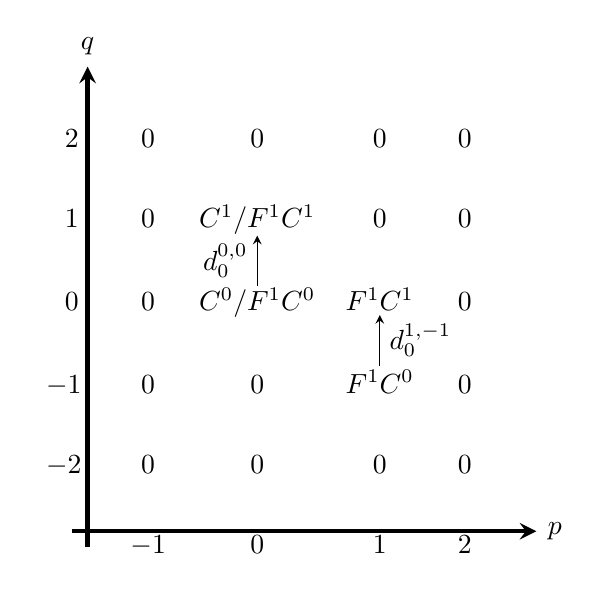
\begin{tikzpicture}[ampersand replacement=\&]
	\matrix (m) [matrix of math nodes,
	nodes in empty cells, nodes={minimum width=5ex,
	minimum height=5ex, outer sep=-5pt},
	column sep=1ex, row sep=1ex]{
	      \&   \&   \&  \&   \& \\
	    2 \& 0 \& 0 \& 0 \& 0 \& \\
	    1 \& 0 \& C^{1}/F^{1}C^{1} \& 0 \& 0 \& \\
	    0 \& 0 \& C^{0}/F^{1}C^{0} \& F^{1}C^{1} \& 0 \& \\
	    -1\hspace{2mm} \& 0 \& 0 \& F^{1}C^{0} \& 0 \& \\
	    -2\hspace{2mm} \& 0 \& 0 \& 0 \& 0 \& \\
	    \quad\strut \& -1 \& 0 \& 1 \& 2 \& \strut \\};
	\draw[-stealth] (m-4-3.north) -- node [left] {$d^{0,0}_{0}$}(m-3-3.south);
	\draw[-stealth] (m-5-4.north) -- node [right] {$d^{1,-1}_{0}$}(m-4-4.south);
	\draw[-stealth, ultra thick] (m-7-1.east) -- (m-1-1.east) node[above]{$q$};
	\draw[-stealth, ultra thick] (m-7-1.north) -- (m-7-6.north) node[right]{$p$};
    \end{tikzpicture}
    \end{column}
    \begin{column}{0.5\textwidth}
	\begin{itemize}
	    \item Since $F^{1}C\subseteq C$ is a subcomplex, $d^{0}\colon C^{0}\to C^{1}$ induces a morphism $d^{0,0}_{0}\colon C^{0}/F^{1}C^{0}\to C^{1}/F^{1}C^{1}$.
	    \item For the same reason, $d^{0}|_{F^{1}C}$ has image in $F^{1}C^{1}$, so we may see it as a morphism
		\[ d_{0}^{1,-1}\colon F^{1}C^{0}\to F^{1}C^{1}. \]
	\end{itemize}
    \end{column}
    \end{columns}
\end{frame}

\begin{frame}
    \frametitle{References}
    \bibliographystyle{alpha}
    \bibliography{main.bib}
\end{frame}
 
\end{document}
